\usepackage{tikz}
\usetikzlibrary{shapes.multipart,positioning}

\usepackage{listings}
\lstdefinelanguage{JavaScript}{
  keywords={typeof, new, true, false, catch, function, return, null, catch, switch, var, if, in, while, do, else, case, break},
  ndkeywords={class, export, boolean, throw, implements, import, this},
  sensitive=false,
  comment=[l]{//},
  morecomment=[s]{/*}{*/},
  morestring=[b]',
  morestring=[b]"
}

\lstset{%
  language=JavaScript,
  basicstyle=\ttfamily,%
  keywordstyle=\bfseries\color{yellow!80!black},%
  ndkeywordstyle=\color{blue!50!white},%
  stringstyle=\color{green},%
  commentstyle=\itshape\color{white!70!black},%
  showstringspaces=false,%
  upquote=true}
% german umlauts
\lstset{
  literate={ö}{{\"o}}1
           {ä}{{\"a}}1
           {ü}{{\"u}}1
           {ß}{{\ss}}1
} 

\title{Objektorientierte Programmierung mit JavaScript}

\author{Malte Schmitz}

\date{16. November 2012}

\begin{document}

\begin{frame}[fragile,plain]
  \begin{center}
    \LARGE Objektorientierte Programmierung \\ mit JavaScript 
  \end{center}
  
  \vskip4ex
  
  \begin{columns}
  \column{7.5em}
  \column{40em}
  \begin{lstlisting}[gobble=4]
    var meta = {
      author: "Malte Schmitz",
      date: new Date(2012, 10, 16),
      event: "MetaNook"
    }
  \end{lstlisting}
  \end{columns}
\end{frame}

\section*{Inhalt}

\begin{frame}{Ziele}
  \begin{enumerate}
    \item JavaScript-Objekte und -Funkionen verwenden können
    \item prototypische (differenzielle) Vererbung verstehen
    \item Objektorientierte Konzepte in JavaScript kennen lernen
    \item sehen, wie JavaScript-Frameworks diese umsetzen
  \end{enumerate}
\end{frame}

\begin{frame}{Gliederung}
  \begin{enumerate}[{Teil} I]
    \item Einführung in JavaScript
    \item Objektorientierung mit JavaScript
    \item Objektorientierung mit JavaScript-Frameworks
  \end{enumerate}
\end{frame}

\begin{frame}{Github}
  \url{github.com/malteschmitz/js-oop}
  \begin{itemize}
    \item diese Präsentation
    \item alle Beispiele
  \end{itemize}
\end{frame}

\section{JavaScript}

\subsection{Objekte}

\begin{frame}[fragile]{Variablen}
  \begin{itemize}
    \item dynamische Typisierung, \emph{nicht} ungetypt
    \item statische (lexikalische) Bindung
    \item Sichtbarkeitsbereich: ganze aktuelle Funktion
  \end{itemize}
  
  \begin{lstlisting}[gobble=4]
    var a; // Deklaration
    console.log(a); // --> undefined
    
    a = 42; // Initialisierung
    console.log(a); // --> 42
    
    // b ist hier bereits deklariert,
    // aber nicht initialisiert
    console.log(b); // --> undefined
    var b = 23; // Deklaration und Initialisierung
  \end{lstlisting}  
\end{frame}

\begin{frame}[fragile]{Kontrollstrukturen}
  \begin{lstlisting}[gobble=4]
    var x = 13;
    while (x < 15) {
      console.log(x); // --> 13, 14
      x += 1;
    }
    if (x >= 15) {
      console.log(x); // --> 15
    }
  \end{lstlisting}
\end{frame}

\begin{frame}[fragile]{Objekte}
  \begin{itemize}
    \item \emph{keine} Instanz einer Klasse
    \item dynamische Sammlung von Eigenschaften (Hash, Map, \ldots)
    \item alles ist ein Objekt
  \end{itemize}
    
  \begin{lstlisting}[gobble=4]
    // Objekt erzeugen
    var o = {};
    
    // Eigenschaft setzen
    o.foo = 42;
    
    // Eigenschaft auslesen
    console.log(o.foo); // --> 42
    
    // Eigenschaft löschen
    delete o.foo;
  \end{lstlisting}  
\end{frame}

\begin{frame}[fragile]{Objektliterale}
  \begin{lstlisting}[gobble=4]
    var meta = {
      author: "Malte Schmitz",
      date: new Date(2012, 10, 16),
      event: "MetaNook"
    }
  \end{lstlisting}
\end{frame}

\begin{frame}[fragile]{Iteration über Objekteigenschaften}
  \begin{lstlisting}[gobble=4]
    for (var key in meta) {
      var value = meta[key];
      console.log(key + ': ' + value);
    }
  \end{lstlisting}
\end{frame}

\begin{frame}[fragile]{\texttt{\&\&} und \texttt{||}}
  \begin{lstlisting}[gobble=4]
    // guard operator
    var author = meta && meta.author;
    
    // default operator
    var obj = meta || {};
  \end{lstlisting}
\end{frame}

\begin{frame}[fragile]{Duck-Typing}
  \begin{quotation}
    When I see a bird that walks like a duck and swims like a duck and
    quacks like a duck, I call that bird a duck.
    
    \raggedleft -- James Whitcomb Riley
  \end{quotation}
  
  \vskip5ex
  
  \begin{lstlisting}[gobble=4]
    if (meta.author) {
      console.log(meta.author);
    }
  \end{lstlisting}
\end{frame}

\begin{frame}[fragile]{globale Variablen}
  \begin{itemize}
    \item Eigenschaften des globalen Objektes
  \end{itemize}
  
  \begin{lstlisting}[gobble=4]
    this
    window
    window.window
  
    foo = 12;
    // entspricht
    windows.foo = 12;
  \end{lstlisting}
\end{frame}

\subsection{Vererbung}

\begin{frame}{differenzielle Vererbung}
  \begin{itemize}
    \item versteckter Link zum Prototypen
    \item beim Lesen Rückgriff auf Prototypen
    \item alle Objekte erben von \lstinline-Object.prototype-  
  \end{itemize}
\end{frame}  
  
\begin{frame}[fragile]{differenzielle Vererbung}
  \begin{tikzpicture}[shorten >=1pt]
    \uncover<4->{
      \node[inner sep=0pt] (talk) {
        \begin{tabular}{|l|l|}
          \hline
          proto & \\ \hline
          \uncover<6-7>{\lstinline-name-} & \uncover<6-7>{\lstinline-Schmitz-} \\ \hline 
        \end{tabular}
      };
      \node[anchor=south west,inner sep=1pt] at (talk.north west) {\lstinline-talk-};
      \node[circle,draw,fill,inner sep=2pt,xshift=2em,yshift=1.5ex] at (talk.center) (talk dot) {};
    }
    \uncover<2->{
      \node[inner sep=0pt,node distance=1em,right=of talk] (meta) {
        \begin{tabular}{|l|l|}
          \hline
          proto & \\ \hline
          \lstinline-name- & \lstinline-Malte- \\ \hline 
        \end{tabular}
      };
      \node[anchor=south west,inner sep=1pt] at (meta.north west) {\lstinline-meta-};
      \node[circle,draw,fill,inner sep=2pt,xshift=2em,yshift=1.5ex] at (meta.center) (meta dot) {};
      \node[right=of meta dot] (obj) {\lstinline-Object.prototype-};
    }
    \only<4->{\draw[->] (talk dot) edge (meta.west |- talk dot);}
    \only<2->{\draw[->] (meta dot) edge (obj);}
  \end{tikzpicture}
  
  \vskip3ex
  
  \uncover<1->{\lstinline-var meta = \{author: "Malte"\};-}\\
  \uncover<3->{\lstinline-var talk = Object.create(meta);-}\\
  \uncover<5->{\lstinline-talk.author = "Schmitz";-}\\
  \uncover<7->{\lstinline-delete talk.author;-}
  
  \vskip3ex
  
  \begin{overprint}
    \only<1-3,5,7>{\quad}
    \only<4>{\lstinline|console.log(talk.author); // --> Malte|}
    \only<6>{\lstinline|console.log(talk.author); // --> Schmitz|}
    \only<8>{\lstinline|console.log(talk.author); // --> Malte|}
  \end{overprint}
\end{frame}

\subsection{Funktionen}

\begin{frame}[fragile]{Funktionen}
  \begin{lstlisting}[gobble=4]
    var square = function(x) {
      return x * x;
    }
  \end{lstlisting}
\end{frame}

\begin{frame}[fragile]{Funktionen}
  \begin{lstlisting}[gobble=4]
    var sum = function() {
      var s = 0, i = 0;
      for (;i < arguments.length; i++) {
        s += arguments[i];
      }
      return s;
    }
  \end{lstlisting}
\end{frame}

\begin{frame}[fragile]{Currying}
  \begin{onlyenv}<1>
    \begin{lstlisting}[gobble=6]
      var add = function(a,b) {
        return a + b;
      }
      var inc = curry(add,1);
      console.log(inc(6)); // --> 7
    \end{lstlisting}
  \end{onlyenv}
  
  \begin{onlyenv}<2>
    \begin{lstlisting}[gobble=6]
      var curry = function(func) {
        var fixed = makeArray(arguments).slice(1);
        return function() {
          var args = makeArray(arguments);
          return func.apply(null, fixed.concat(args));
        }
      }
    \end{lstlisting}
  \end{onlyenv}
\end{frame}

\subsection{Funktionsaufrufe}

\begin{frame}{Funktionsaufrufe}
  \begin{tabular}{ll}
    Aufruf & \lstinline-this- \\ \hline
    \lstinline-sum()- & globales Object \\
    \lstinline-obj.sum()- & \lstinline-obj- \\
    \lstinline-sum.apply(foo)- & \lstinline-foo- \\
    \lstinline-new sum()- & neues Object
  \end{tabular}
\end{frame}

\begin{frame}[fragile]{Funktionsaufrufe}
  \begin{lstlisting}[gobble=4]
    sum(1,2,3);
    sum.apply(window, [1, 2, 3]);
    sum.call(window, 1, 2, 3);
    
    
    meta.add = sum;
    
    meta.add(1,2,3);
    sum.apply(meta, [1, 2, 3]);
    sum.call(meta, 1, 2, 3);
  \end{lstlisting}
\end{frame}

\begin{frame}[fragile]{\lstinline-new--Operator}
  \begin{lstlisting}[gobble=4]
    var a = new Fun(42);
  
  
    var a = Object.create(Fun.prototype);
    a.constructor = Fun;
    var res = Fun.call(a, 42);
    if (res && (typeof res === 'object' ||
                typeof res === 'function')) {
      a = res;
    }
  \end{lstlisting}
\end{frame}

\begin{frame}[fragile]{Iteration über Objekteigenschaften}
  \begin{lstlisting}[gobble=4,basicstyle=\small\ttfamily]
    for (var key in meta) {
      if (Object.prototype.hasOwnProperty.apply(key)) {
        var value = meta[key];
        console.log(key + ': ' + value);
      }
    }
  \end{lstlisting}
\end{frame}

\begin{frame}[fragile]{\lstinline-makeArray-}
  \begin{lstlisting}[gobble=4]
    var makeArray = function(a) {
      return Array.prototype.slice.call(a);
    }
  \end{lstlisting}  
\end{frame}

\begin{frame}[fragile]{\lstinline-Object.create-}
  \begin{lstlisting}[gobble=4]
    if (typeof Object.create !== 'function') {
      Object.create = function(obj) {
        var F = function(){};
        F.prototype = obj;
        return new F();
      }
    }
  \end{lstlisting}  
\end{frame}

\section{Objektorientierung}

\subsection{pseudoklassische Vererbung}

\begin{frame}
  no content
\end{frame}

\subsection{prototypische Vererbung}

\begin{frame}
  no content
\end{frame}

\subsection{funktionale Vererbung}

\begin{frame}
  no content
\end{frame}

\subsection{Vererbung durch Kopieren}

\begin{frame}
  no content
\end{frame}

\section{Frameworks}

\begin{frame}
  no content
\end{frame}

\subsection{Underscore.js und \texttt{\_.extend}}

\begin{frame}
  no content
\end{frame}

\subsection{jQuery und \texttt{\$.extend}}

\begin{frame}
  no content
\end{frame}

\subsection{YUI und \texttt{Y.extend}}

\begin{frame}
  no content
\end{frame}

\subsection{Backbone.js und \texttt{Backbone.Model.extend}}

\begin{frame}
  no content
\end{frame}

\subsection{MooTools und \texttt{new Class}}

\begin{frame}
  no content
\end{frame}

\subsection{Prototype und \texttt{Class.create}}

\begin{frame}
  no content
\end{frame}

\section*{Zusammenfassung}

\begin{frame}{Zusammenfassung}
  \begin{itemize}
    \item \alert{Prototypische/differenzielle Vererbung} ist eine \alert{Verallgemeinerung} der
      klassenbasierten Verberbung.
    \item \alert{Klassenbasierte Vererbung} kann in JavaScript \alert{simuliert} werden.
    \item Es muss zwischen \alert{prototypischer Vererbung} und \alert{Vererbung durch
      Kopieren} unterschieden werden.
    \item In der Praxis sucht man sich eines der \alert{vielen Frameworks} für
      \alert{Objektorientierte Programmierung mit JavaScript}.
  \end{itemize} 
\end{frame}

\begin{frame}{Crockford on JavaScript}
  \begin{thebibliography}{1}
    \bibitem{1} Volume One:
    \emph{The Early Years}
    \newblock 25. Januar 2010
    
    \bibitem{2} Chapter 2:
    \emph{And Then There Was JavaScript}
    \newblock 5. Februar 2010
    
    \bibitem{3} Act III:
    \emph{Function the Ultimate}
    \newblock 17. Februar 2010
    
    \bibitem{4} Episode IV:
    \emph{The Metamorphosis of Ajax}
    \newblock 3. März 2010
    
    \bibitem{5} Part 5:
    \emph{The End of All Things}
    \newblock 31. März 2010
    
    %\bibitem{6} Scene 6:
    %\emph{Loopage}
    %\newblock 27. August 2010
    %
    %\bibitem{7} Level 7:
    %\emph{ECMAScript 5: The New Parts}
    %\newblock 29. März 2011
    %
    %\bibitem{8} Section 8:
    %\emph{Programming Style and Your Brain}
    %\newblock 3. November 2011
  \end{thebibliography}
\end{frame}

\begin{frame}{Bücher}
  \begin{thebibliography}{1}
    \bibitem{1} David Flanagan
    \newblock \emph{JavaScript: The Definitive Guide}
    
    \bibitem{2} Douglas Crockford
    \newblock \emph{JavaScript: The Good Parts}
  \end{thebibliography}
\end{frame}

\end{document}